\section{System Overview}
Through the system overview diagram, in figure \ref{fig:system_overview}, it is possible to identify the main modules of the system to be developed, and how they interact. We can divide the system into three subsystems: the local system, which represents a lamppost, the gateway system, device connected to the lampposts network and to the remote server, and the remote system, that stores information about the lamppost network and allows interaction with the system users by remote client applications.

\begin{figure}[H]
	\centering
	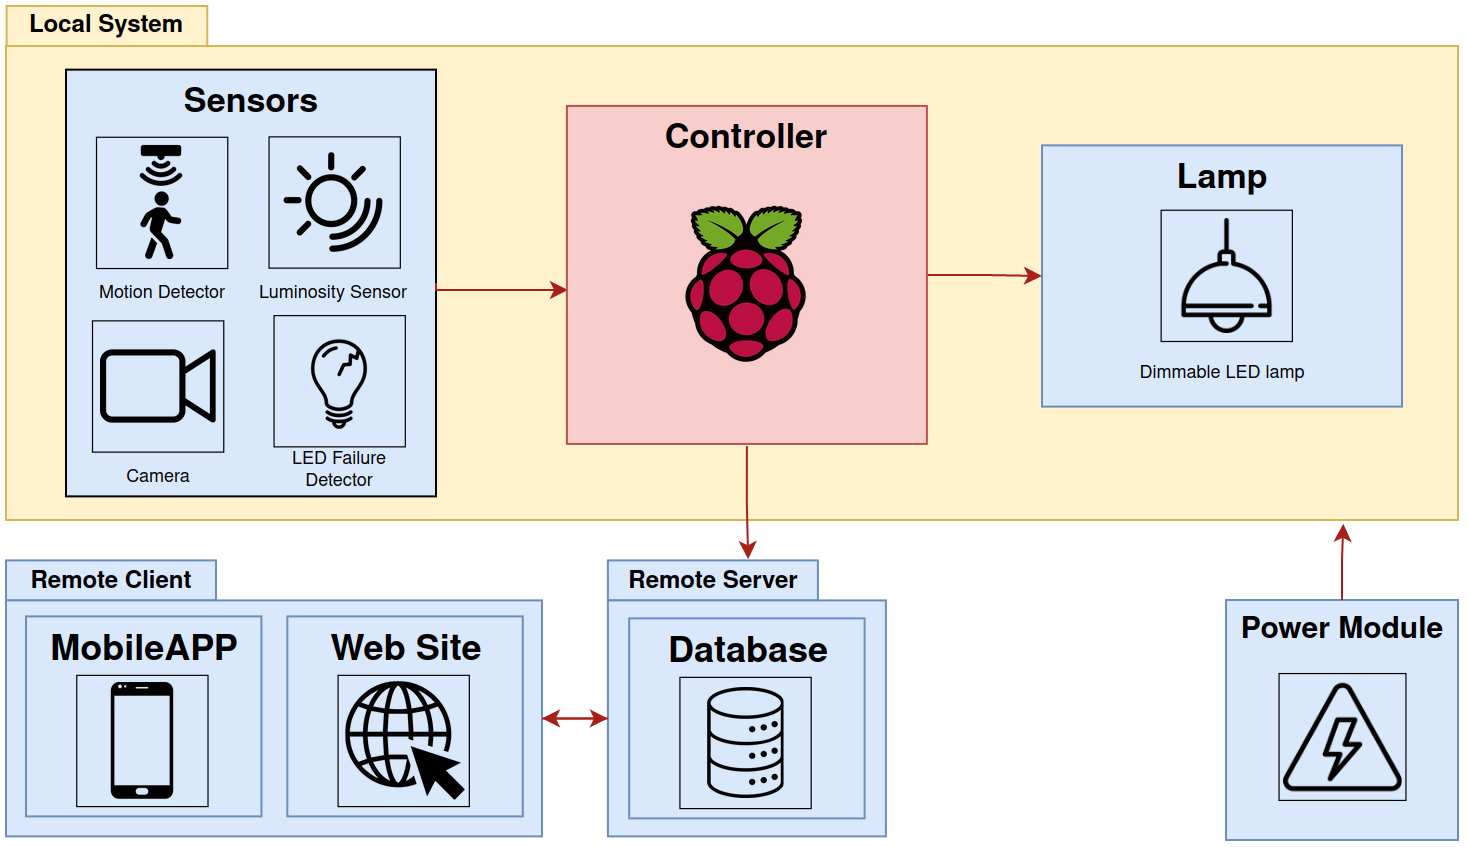
\includegraphics[width=0.92\textwidth]{03system_overview/system_overview}
	\caption{System Overview Diagram.}
	\label{fig:system_overview}
\end{figure}

The local system is composed of sensors, a controller, a lamp and a wireless communication module. Regarding the sensors, there will be a motion detector, to allow the detection of movement in the vicinity of the pole, a luminosity sensor, to detect the light conditions of the pole’s surroundings, a lamp failure detector to know if the lamp is working and a camera to detect empty parking spots in the lamppost vicinity. The controller of the local system is a Raspberry Pi, that use the sensors information and communicate wirelessly with the gateway using a LoRa communication module, so that the lights are dinamically turned on. The gateway controller also communicates through internet with a remote server.

The remote system is composed by the remote server and the remote client. The remote server consists of a database that stores all information about each lamp post location and operating status. This information can be accessed through a mobile application by the operator in order to carry out the necessary maintenance of the lamp of each pole. Furthermore, the operator, when installing a new lamppost, can add its location to the database, using the mobile application. In addition, the database stores information on available parking spaces detected by the camera. When a user, a car driver, wants to know where there are empty parking places, he can access a website that informs him of the location of the empty parking spaces.

Knowing that the public lighting network is directly related to the electrical network, this will be used to power each local system.

\section{System Architecture}
Using the system overview diagram information, one can describe the system in two different architectures. Hardware architecture, as how the hardware modules interfaces with itself, what are the physical components of the system, and software architecture, which details how the information is processed among different software layers. In this section, it will only be referenced the architectures of the base station, since the local system architecture is similar, as seen previously. 

\subsection{Hardware Architecture}

\subsubsection{Local System}

In figure \ref{fig:local_hw_arch}, one can see the diagram that represents the physical connections of the system. The Raspberry Pi is the main component in the system, processing all the information given by the sensors, via \ac{gpio} pins and \ac{csi} for the camera. The communication between the Raspberry Pi and the LoRa module is done by \ac{spi} protocol.
%, and also controlling the \ac{led} lamp brightness. 
The power of all system components comes from the power grid and, through an AC/DC converter, will power the Raspberry Pi and its associated sensors.
In order to power the lamp and at the same time control its brightness, a driver is used, taking the controller output, a \ac{pwm} signal, and system power as inputs. 

%\clearpage 
\begin{figure}[ht]
	\centering
	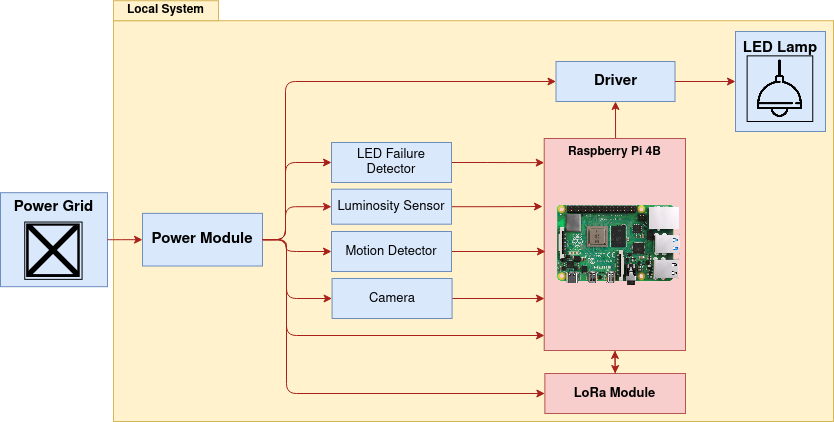
\includegraphics[width=.75\textwidth]{03system_overview/local_hw_arch}
	\caption{Local System Hardware Architecture Diagram.}
	\label{fig:local_hw_arch}
\end{figure}

\subsubsection{Gateway}

The hardware achitecture of the gateway is shown in figure \ref{fig:gateway_hw_arch}. The purpose of this device is communicate with the local systems and control a network of street lampposts, so the hardware needed to complete these tasks is only the LoRa communication module that uses \ac{spi} to interface with the Raspberry Pi, the gateway controller.

%\clearpage 
\begin{figure}[ht]
	\centering
	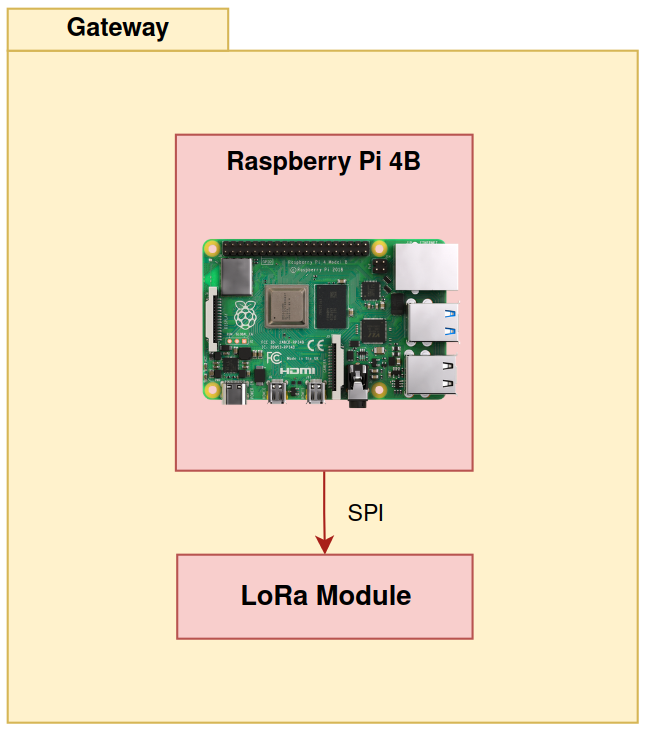
\includegraphics[width=.45\textwidth]{03system_overview/gateway_hw_arch}
	\caption{Gateway Hardware Architecture Diagram.}
	\label{fig:gateway_hw_arch}
\end{figure}

\subsection{Software Architecture}
The software architecture is divided into three layers:
\begin{itemize}
        \item The \textbf{Operating System} layer, which is composed by the Operating System drivers and Board Support Packages;
        \item The \textbf{Middleware} layer, which includes software for abstracting the lower level layer packages. It works as a pipe since it links two applications, in different layers, so that data can be easily transmitted;
        \item The \textbf{Application} layer, where the core functionality of the program is built, with a resource for the API's in the lower level layers.
\end{itemize}

\subsubsection{Local System}

As shown in figure \ref{fig:local_sw_arch}, the operating system layer is composed by the sensor drivers, such as the LED Failure Sensor, the Luminosity Sensor, the Motion Detector which uses \ac{gpio} drivers, the camera, that uses \ac{csi} drivers and also the LoRa Communication driver. In the middleware layer are the tools needed to process the images from the camera, to multitasking, using PThreads execution model, to acquire data from sensors and to communicate via LoRa protocol with the gateway. The application layer manages the communication with the gateway.

\begin{figure}[H]
	\centering
	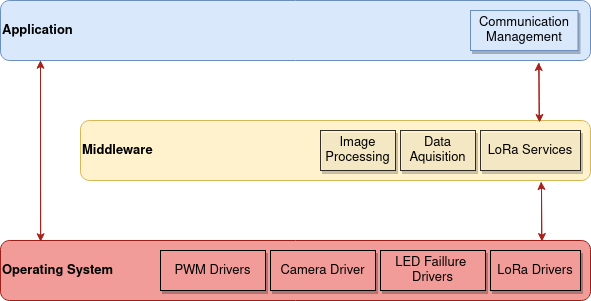
\includegraphics[width=.85\textwidth]{03system_overview/local_sw_arch}
	\caption{Local System Software Architecture Diagram.}
	\label{fig:local_sw_arch}
\end{figure}

\subsubsection{Gateway}

In figure \ref{fig:gateway_sw_arch} is shown the software architecture of gateway device. The operating system layer is composed by the LoRa communication device driver, whose interface is done using \ac{spi} protocol. The middleware layer deals with the PThreads execution model, in order to have multitasking, and the LoRa protocol services. Finally, the application layer manages the system database, as well as the \ac{gui}, that is the mobile application and the web site, and also all communications with the neighbor street poles.

\begin{figure}[H]
	\centering
	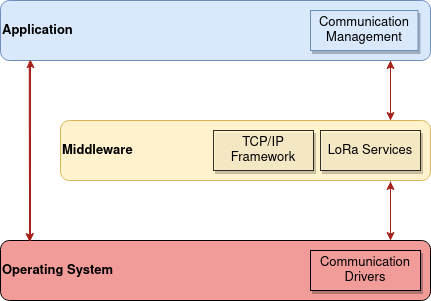
\includegraphics[width=.75\textwidth]{03system_overview/gateway_sw_arch}
	\caption{Gateway Software Architecture Diagram.}
	\label{fig:gateway_sw_arch}
\end{figure}

\clearpage
\subsection{Database E-R Diagram}
In the database will be stored all the information about each lamppost, its operators and parking spots. In the figure \ref{fig:Database} one can see the Entity Relationship Diagram (E-R Diagram) that displays the relationships between the entities, that is the things of interest in this specific domain of knowledge. This database has five entities: Lamppost, Location, Region, Operator and Parking Space. A lamppost have a unique identification, his location coordinates and the status of the lamp (light dimmed/ light fully ON/ OFF/ broken). The location is defined by the coordinates, the post code associated and the street name. A region has multiple locations associated, that are defined by the post code. This entity has also information about parish, county, district of the specified region and the operator responsible for the lampposts in that region. The entity operator has the operator identification and the operator name. A parking spot is defined by the entity Parking Space and has the attributes identification of the parking space, its location coordinates, the parking space type (normal park/ park for disabled people/ restrict park) and the park status (taken/ not taken).

%\subsubsection{Relational Model}
%
%lamppost(\uline{pole\_id}, \dotuline{gps}, pole\_status)
%
%location(\uline{gps}, \dotuline{post\_code}, street\_name)
%
%region(\uline{post\_code}, \dotuline{operator\_id}, parish, county, district)
%
%operator(\uline{operator\_id}, operator\_name)
%
%parking\_space(\uline{park\_id}, \dotuline{gps}, park\_type, park\_status)

\begin{figure}[ht]
        \centering
        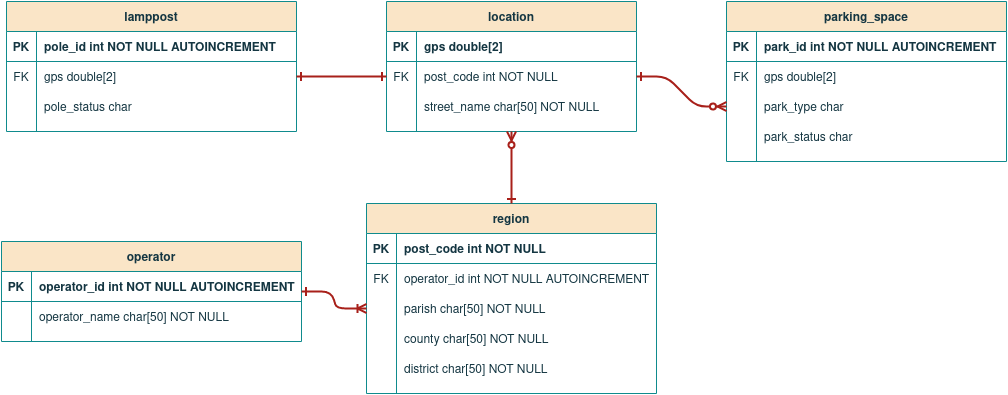
\includegraphics[width=.92\textwidth]{03system_overview/database}
        \caption{Database E-R Diagram.}
        \label{fig:Database}
\end{figure}

